\documentclass[12pt, a4paper]{article}

\usepackage[utf8]{inputenc}
\usepackage[T1]{fontenc}
\usepackage{amsmath, amssymb}
\usepackage{graphicx}
\usepackage[margin=1in]{geometry}
\usepackage{hyperref}
\usepackage{booktabs}
\usepackage{xcolor}
\usepackage{float}
\usepackage{caption}
\usepackage{natbib}
\usepackage{microtype}

\hypersetup{
    colorlinks=true,
    linkcolor=blue!60!black,
    citecolor=blue!60!black,
    urlcolor=blue!60!black,
}

\title{Where do the other worlds go?\\
  A toy-model test of Born-rule filtering in a local Ising chain}

\author{Laurent Eschenauer\\
  \small Independent Researcher\\
  \small \href{mailto:laurent@eschenauer.be}{laurent@eschenauer.be}}

\date{\today}

\begin{document}
\maketitle

\begin{abstract}
Strasberg and collaborators reported, in random matrix toy models, a filtering
effect in which Born-atypical frequency classes of quantum histories recohere
while Born-typical ones remain decoherent. We test whether the same qualitative
pattern appears in a physically motivated system: a 9-qubit transverse-field Ising
chain ($D = 512$) with local, nearest-neighbor couplings and exact unitary
evolution. In our model, the recoherence parameter $\varepsilon$ dips near the
Born frequency ($n_1/L \approx p_1 = 0.746$) with a $3.1\times$ gap over the
combinatorial peak, averaged over 10 Haar-random initial states, matching the
qualitative shape of the random matrix prediction. At the individual-branch level
($L = 12$, 4096 branches), only 451 branches remain approximately decoherent
($\varepsilon < 0.3$), and these cluster at Born-typical frequencies.
In this toy model, the Born-typical filtering pattern emerges from the interplay
of finite dimensions and local unitary dynamics---though whether this generalizes
beyond toy models remains open.
\end{abstract}


% ============================================================================
\section{Introduction}
\label{sec:intro}
% ============================================================================

Quantum mechanics has a puzzle at its core, and it is surprisingly easy to state.

The Schr\"odinger equation is deterministic and linear. If you know the state of a
system right now, you can compute its state at any future time---no randomness, no
choices, no collapse. And yet, every time we open the box and look at the cat, we
see one definite outcome. The math says the cat is in a superposition of alive and
dead. Our eyes say it is one or the other.

This is the measurement problem, and it has been with us since the 1920s. There is
no shortage of proposed solutions. The Copenhagen interpretation says the wave
function collapses upon measurement, but never quite explains what counts as a
measurement. Bohmian mechanics adds hidden variables. Objective collapse theories
add new physics. And then there is Everett's proposal~\citep{Everett1957}: nothing
collapses at all. The Schr\"odinger equation is the whole story. What we experience
as ``collapse'' is the universe splitting into branches---every possible outcome
happens, each in its own branch of reality, and we simply find ourselves in one of
them.

The Everett picture is elegant, but it raises its own question. If every outcome
happens, why do we observe outcomes with the frequencies predicted by the Born rule?
If there is one branch where the electron goes left and one where it goes right,
and both are equally real, why do we not see 50/50 statistics regardless of the
quantum state?

This is sometimes called the \emph{probability problem} of the many-worlds
interpretation, and it is the subject of a large literature.
Deutsch~\citep{Deutsch1999} gave the first decision-theoretic argument:
a rational agent in a branching universe \emph{should} weight branches by their
squared amplitudes. Wallace~\citep{Wallace2012} refined and extended the proof;
Carroll~\citep{Carroll2019} offers an accessible account and argues,
with Sebens, that Born's rule follows from self-locating uncertainty at the
moment of branching.
Zurek~\citep{Zurek2005} pursued a different strategy, deriving Born's rule from
environment-assisted invariance (``envariance'') without decision theory.
These approaches are persuasive to some and unconvincing to others. What they share
is that they introduce additional postulates---rationality axioms or
symmetry principles---beyond the Schr\"odinger equation itself.

Recently, Strasberg and collaborators~\citep{Strasberg2024, StrasbergSchindler2024,
Strasberg2025} have explored a different route. Their argument is physical, not
decision-theoretic. In a finite-dimensional Hilbert space, the histories of a
quantum system cannot all remain decoherent as the number of branching events grows.
There are more histories than dimensions, so branches must start overlapping.
In random matrix toy models, they reported that this overlap is not uniform: the
histories whose frequencies match the Born rule remain decoherent, while the others
do not. Whether this filtering pattern is a generic feature of finite-dimensional
quantum mechanics or specific to the models studied remains an open question.

Strasberg's results are established for random matrix Hamiltonians and related
asymptotic arguments. We ask: does the same qualitative behavior appear in a
concrete, physically motivated Hamiltonian? We take a 9-qubit transverse-field Ising
chain---a nearest-neighbor spin model near its critical point---and check.


% ============================================================================
\section{The Puzzle: All Branches Exist, but the Statistics Are Wrong}
\label{sec:puzzle}
% ============================================================================

Take a loaded coin: 75\% heads, 25\% tails. We know what probability means here.
Flip it many times, and about 75\% of the flips will come up heads. That is what
we observe. That is what we mean by the coin being ``loaded.''

Now flip it once in the Everett picture. Both outcomes happen. There are two
branches: one where you got heads, one where you got tails. Both are real. Both
exist. So what does ``75\% probability'' even mean, if both outcomes occur with
certainty?

Flip again. Now there are four branches: HH, HT, TH, TT. All four exist. Of
these, one has 0 heads, two have 1 head, and one has 2 heads. If you just count
branches, the most common outcome is 50\% heads---not 75\%.

After three flips, there are 8 branches. The branch-counting peak is still at
50\% heads. After ten flips, there are 1024 branches, and $\binom{10}{5} = 252$
of them have exactly 50\% heads, while only $\binom{10}{7} = 120$ have 70\% heads.
The more you flip, the worse it gets: branch counting says 50\%, but we observe
75\%.

This is the probability problem of the many-worlds interpretation. If every branch
is equally real, what does probability mean? And why do we see the loaded-coin
statistics instead of the branch-counting statistics?


% ============================================================================
\section{Background: Recoherence in Finite Hilbert Space}
\label{sec:background}
% ============================================================================

The key is that Hilbert space is finite.

A quantum system with $m$ qubits lives in a Hilbert space of dimension $D = 2^m$.
Think of this as a pond with a fixed surface area. Each branch of the wave function
is a lily pad. After $L$ coin flips, there are $2^L$ lily pads. When $L$ is small,
there is plenty of room---each pad has its own patch of water, and they do not
interfere. But the pond is finite. When $2^L > D$, the pads are competing for the
same surface. They crowd, overlap, and shade each other out. Not all can survive
as distinct plants.

In quantum language, branches that ``overlap'' are no longer orthogonal. Their
quantum states point in nearly the same direction, which means they cannot be
distinguished by any measurement. They have lost their identity as separate
worlds. This language draws on the decoherent (or consistent) histories
framework~\citep{Griffiths1984, GellMannHartle1990}, in which a set of histories
counts as ``classical'' only when their mutual overlaps are negligible.
Following Strasberg~\citep{Strasberg2025}, we call the loss of this condition
\emph{recoherence}---the opposite of decoherence.

Strasberg and collaborators~\citep{StrasbergSchindler2024, Strasberg2025}
reported that, in their random matrix models, this competition is not democratic.
The branches that get shaded out are not random.
They are the ones near 50\% heads---the branch-counting peak. The branches near
75\% heads---the Born frequency---remain more nearly decoherent.

\subsection{Measuring Decoherence}

To make this precise, we need a way to measure how much two branches overlap.

We group branches by their frequency---the total number of heads $n_1$ out of $L$
flips. The frequency-class state $|\psi(n_1)\rangle$ is the quantum state
obtained by adding up all branches that got exactly $n_1$ heads:
\begin{equation}
  \label{eq:freq-class}
  |\psi(n_1)\rangle = \sum_{\mathbf{x}:\, n_1(\mathbf{x}) = n_1}
    \Pi_{x_L} U_L \cdots \Pi_{x_1} U_1 |\Psi_0\rangle,
\end{equation}
where $U_k$ is the evolution between flips and $\Pi_{x_k}$ picks out the
heads-or-tails outcome at flip $k$.

The \emph{recoherence parameter}
$\varepsilon$~\citep{StrasbergSchindler2024} measures how much a frequency class
overlaps with any other frequency class---a score from 0 to 1:
\begin{equation}
  \label{eq:epsilon}
  \varepsilon(n_1) = \max_{n_1' \neq n_1}
    \frac{|\langle\psi(n_1')|\psi(n_1)\rangle|}
         {\sqrt{\langle\psi(n_1)|\psi(n_1)\rangle \cdot \langle\psi(n_1')|\psi(n_1')\rangle}}.
\end{equation}
At $\varepsilon = 0$, the frequency class is fully decoherent (orthogonal to all
others). At $\varepsilon = 1$, it is fully recoherent (indistinguishable from
another class).

\subsection{The Prediction}

In their random matrix toy models, Strasberg and collaborators found that, as the
number of flips $L$ grows:
\begin{itemize}
  \item Frequency classes near 75\% heads have low $\varepsilon$---they stay decoherent,
  \item frequency classes near 50\% heads have high $\varepsilon$---they blur together,
  \item the gap grows with $L$.
\end{itemize}
The pond is too small for all the lily pads near 50\%. They shade each other out.
The ones near 75\% remain more nearly decoherent.


% ============================================================================
\section{Numerical Experiment}
\label{sec:experiment}
% ============================================================================

We simulate repeated coarse-grained measurements on a 9-qubit Ising chain and
analyze the decoherence structure of the resulting
branches.\footnote{All simulation code is available at
\url{https://github.com/eschnou/quantum-recoherence}.}

The setup can be thought of as a loaded quantum coin flip repeated $L$ times.
The coin comes up heads 75\% of the time. In the many-worlds picture, every
outcome sequence occurs as a branch. We track all $2^L$ branches and compute the
recoherence parameter $\varepsilon$ for each, asking: which branches remain
approximately decoherent, and which lose their identity through overlap with
neighbors?

\subsection{Setup: The Ising Chain}
\label{sec:setup}

We use 9 qubits arranged in a line, interacting through the transverse-field Ising
Hamiltonian:
\begin{equation}
  H = \frac{J}{2} \sum_{i=0}^{7} Z_i Z_{i+1}
    + h_x \sum_{i=0}^{8} X_i,
\end{equation}
with parameters $J/2 = 0.5$ and $h_x = 0.9045$, placing the system near the
quantum critical point ($h_x/J \approx 0.9$). In this regime, the nearest-neighbor
couplings generate significant entanglement and spreading of correlations. The
Hilbert space has dimension $D = 2^9 = 512$.

Each ``coin flip'' works like this: let the qubits evolve under $H$ for one time
step, then ask a coarse question about the result. Our question is: are at least
4 of the 9 qubits in state $|1\rangle$? If yes, we call it ``heads.'' If no,
``tails.'' Since 382 of the 512 basis states have Hamming weight $\geq 4$, the
coin is loaded: $p_\text{heads} = d_1/D = 382/512 \approx 75\%$, where $d_1$ is
the rank of the ``heads'' projector. In Strasberg's framework, this ratio $d_1/D$
defines the Born-typical frequency: it is the single-trial Born probability
averaged over Haar-random initial states. We verified numerically that our Ising
chain produces effective single-step probabilities consistent with this ratio
($p_1^\text{eff} = 0.747 \pm 0.018$ over 200 Haar-random states).

No actual measurement is performed. The system evolves unitarily, and we apply
the heads/tails decomposition analytically---projecting the state vector onto the
two subspaces without collapsing it.
The 9-qubit system is both the coin and the recorder. There is no separate
environment.

\subsection{Methods}
\label{sec:methods}

Each evolution step applies $U = e^{-iH\Delta t}$ with $\Delta t = 1.2$,
computed via exact matrix exponentiation.

Initial states are drawn Haar-randomly on the full $D$-dimensional Hilbert space.
All frequency-class results are averaged over 10 independent random seeds; error
bars show $\pm 1\sigma$.

Branch-level decoherence counts use the operational threshold
$\varepsilon < 0.3$. This threshold is a conventional choice; the qualitative
conclusion---that survivors cluster at Born-typical frequencies---holds for
thresholds in the range $[0.1, 0.5]$, though the absolute count of
``decoherent'' branches varies.\footnote{Robustness checks (threshold
sensitivity, $\Delta t$ variation) are included in the code repository.}

\subsection{Frequency-Class Results}
\label{sec:freq-results}

We first analyze frequency classes (groups of branches with the same number of
heads), which is cheap enough to run at $L = 15$ flips. We repeat with 10
different random starting states. For each run, we compute $\varepsilon$ for every frequency
class.

Figure~\ref{fig:overlay} shows the result. The frequency classes near 75\% heads
(the Born prediction) have low $\varepsilon$---they remain approximately
decoherent. The classes near 50\% heads (the branch-counting peak) have
$\varepsilon$ approximately three times higher---they overlap significantly with
neighboring classes.

As a sanity check, we also run Strasberg's own random matrix model at the same
dimension and coin loading. The two curves match: the Ising chain reproduces what
random matrix theory predicts.

\begin{figure}[H]
  \centering
  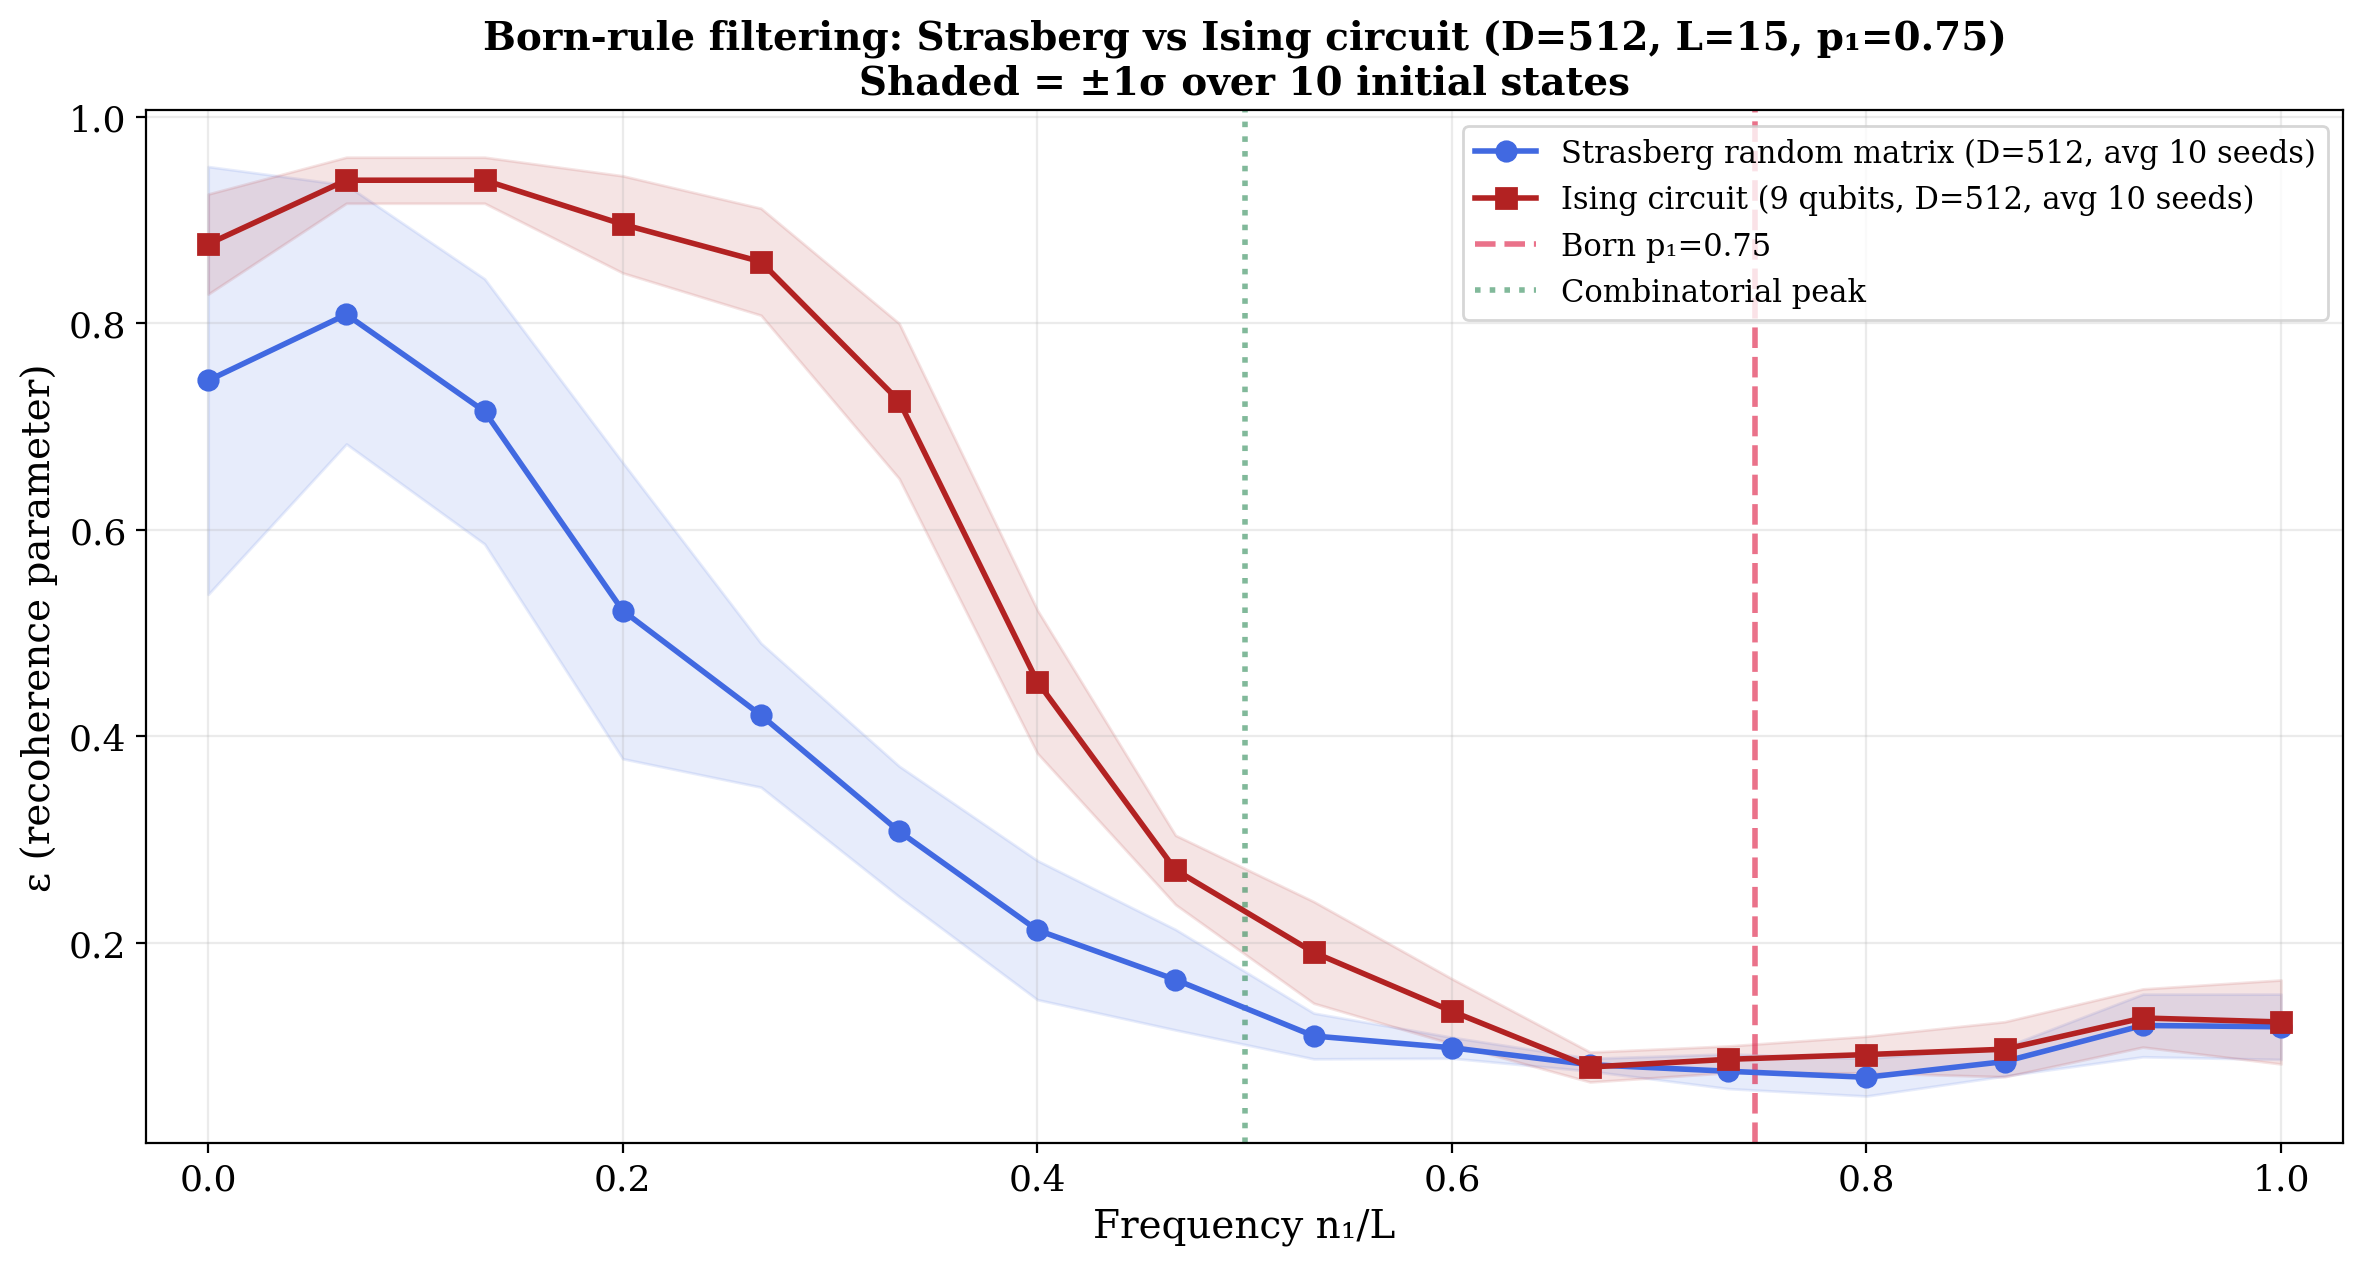
\includegraphics[width=0.95\textwidth]{../results/overlay.png}
  \caption{Recoherence parameter $\varepsilon(n_1/L)$ for the 9-qubit
    transverse-field Ising chain (red, exact matrix exponentiation) and
    Strasberg's random matrix model (blue) at $D = 512$, $L = 15$,
    $p_1 = 0.746$. Averaged over 10 Haar-random initial states; shaded regions
    show $\pm 1\sigma$. Both curves dip near the Born frequency (red dashed)
    and rise toward the combinatorial center (green dotted), showing the same
    qualitative filtering pattern.}
  \label{fig:overlay}
\end{figure}

The result is robust. All 10 seeds show the same qualitative shape. The standard
deviation of $\varepsilon$ across seeds is small relative to the Born--combinatorial
gap, indicating that the effect is a property of the Hamiltonian, not of special
initial states.

\subsection{Branch-Level Analysis}
\label{sec:branches}

So far we have grouped branches by their frequency (how many heads total). But we
can go deeper: track every single branch individually. Each specific sequence of
heads and tails---like HHTHTTHHTTHH---is one branch, one possible history of the
coin. We compute $\varepsilon$ for each one: how much does this branch overlap with
any other?

Figure~\ref{fig:branch-death} shows what happens as we increase the number of
flips. At $L = 4$ (16 branches, 512 dimensions), the pond is nearly empty---almost
every branch is a distinct world. At $L = 9$ (512 branches, 512 dimensions), the
pond is full. At $L = 12$ (4096 branches, 512 dimensions), it is eight times
oversubscribed. Only 451 branches remain approximately decoherent
($\varepsilon < 0.3$). By $L = 13$ (8192 branches), 565 survive---slightly
above $D$, since the threshold $\varepsilon < 0.3$ allows partial overlap.

The survivors cluster at Born-typical frequencies.

\begin{figure}[H]
  \centering
  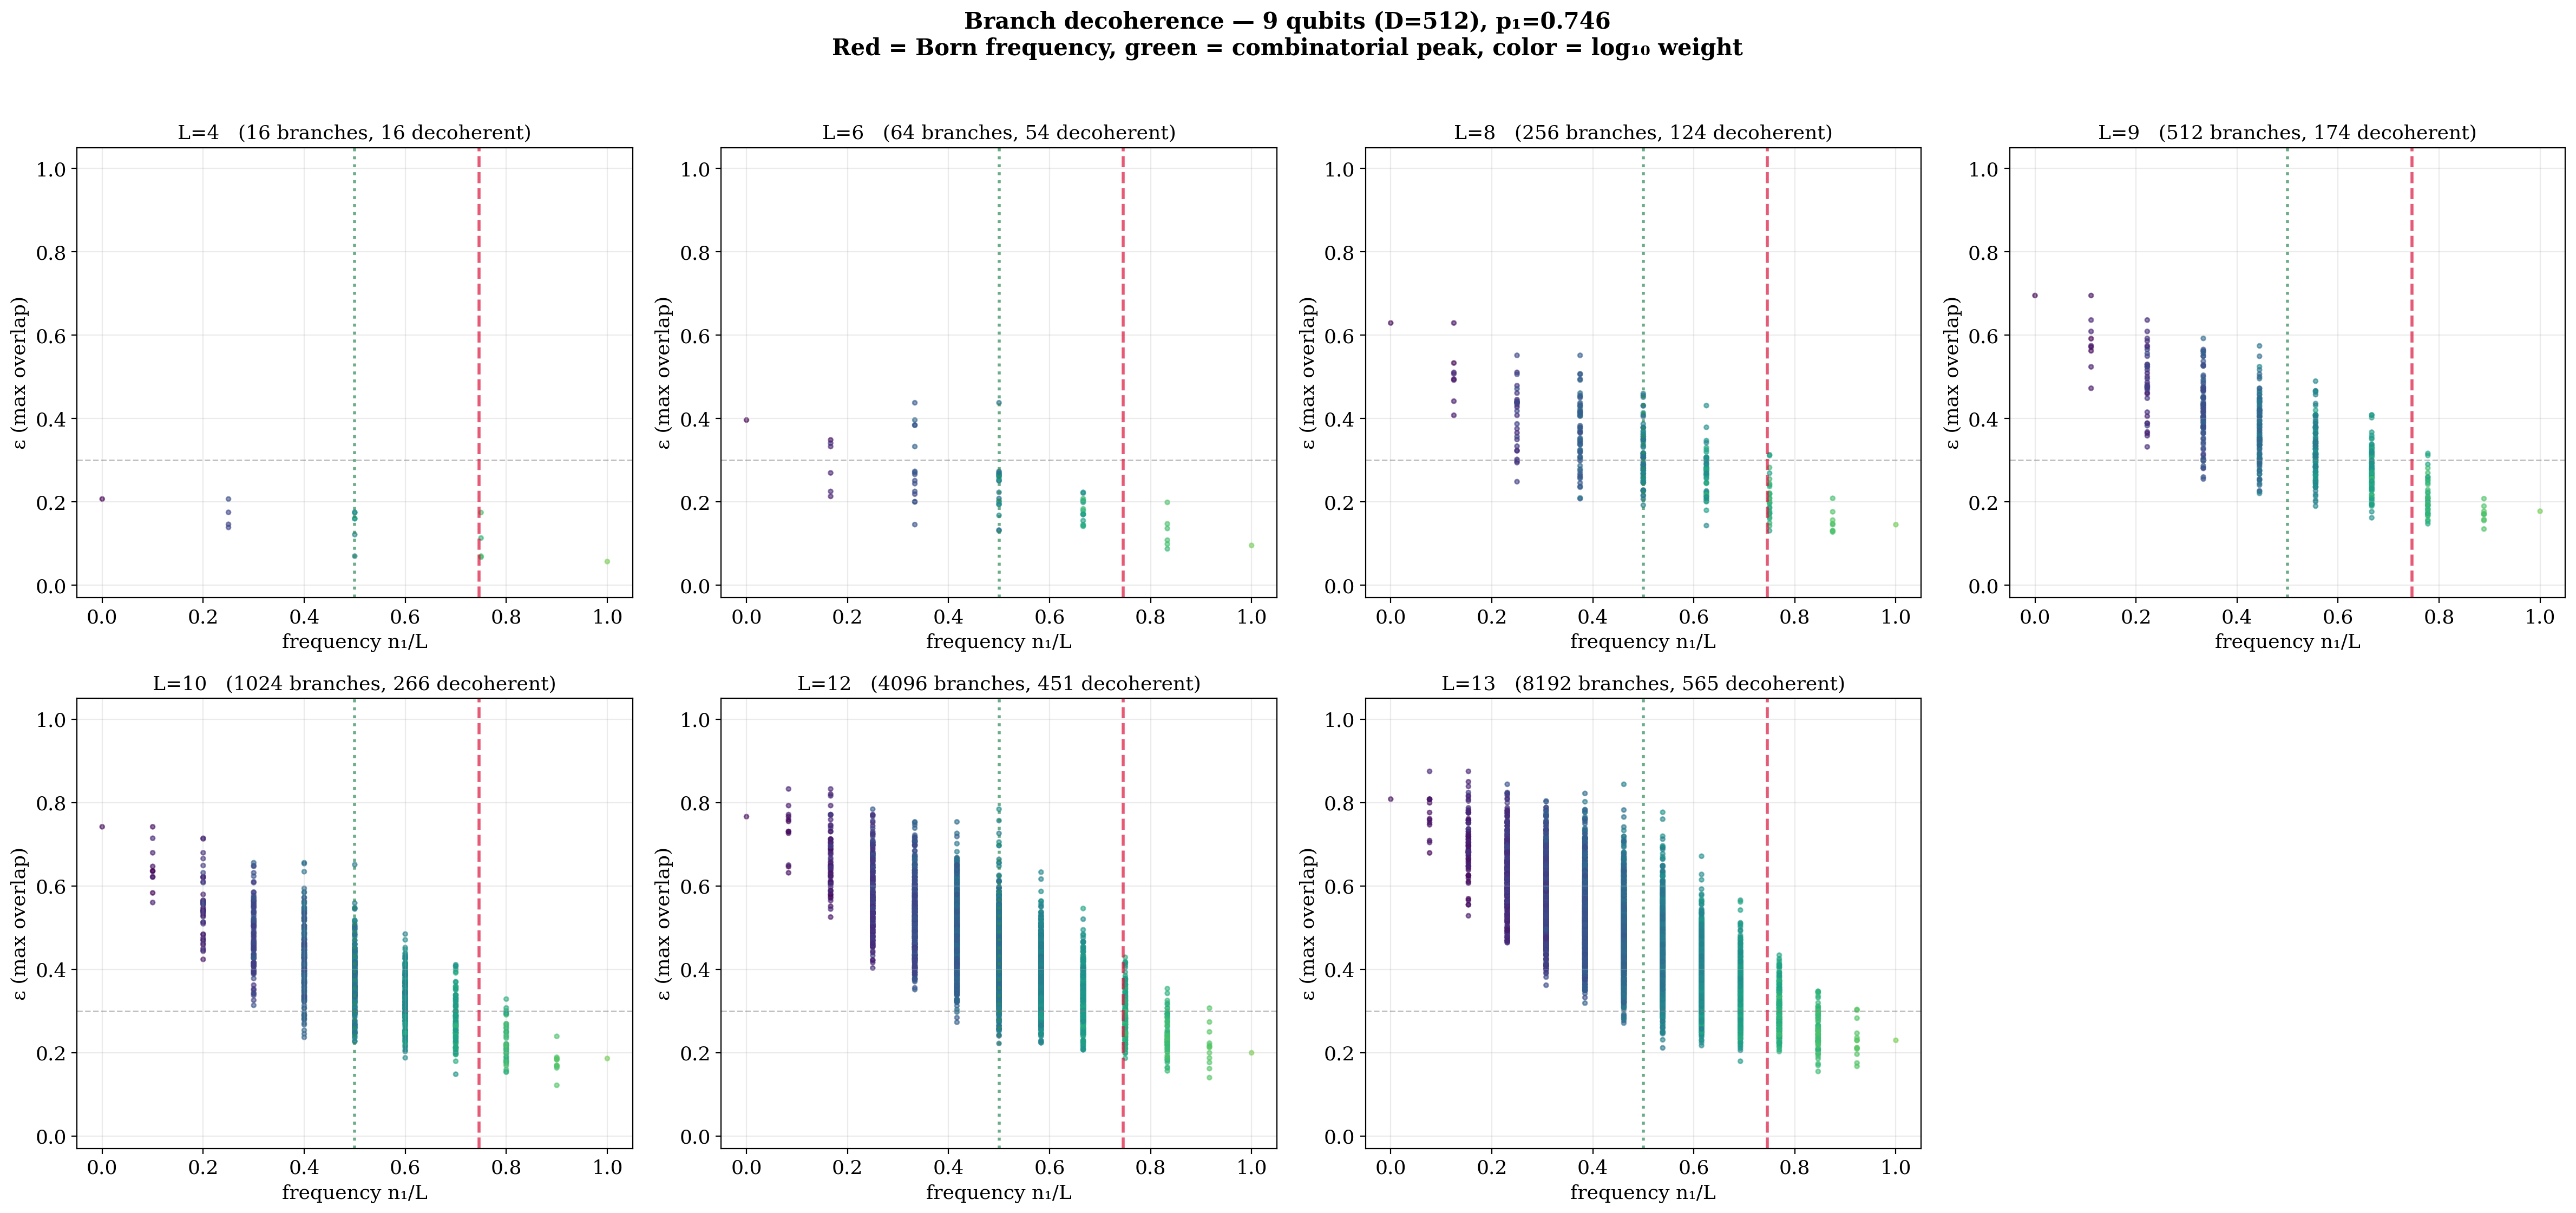
\includegraphics[width=0.95\textwidth]{../results/branch_death.png}
  \caption{Recoherence parameter for individual branches at seven values of $L$.
    Each dot is one of $2^L$ branches; color encodes log weight. The decoherence
    threshold $\varepsilon = 0.3$ is shown as a gray dashed line. At $L = 13$,
    8192 branches compete for 512 dimensions; only 565 satisfy
    $\varepsilon < 0.3$, clustered near the Born frequency (red dashed).}
  \label{fig:branch-death}
\end{figure}

Figure~\ref{fig:census} makes the census explicit. The total number of branches
grows exponentially ($2^L$), but the growth of decoherent branches slows
dramatically around $D = 512$. The dimension $D$ is not a hard ceiling---approximate
decoherence ($\varepsilon < 0.3$) allows more than $D$ coexisting branches---but
it sets the scale at which the competition intensifies.

\begin{figure}[H]
  \centering
  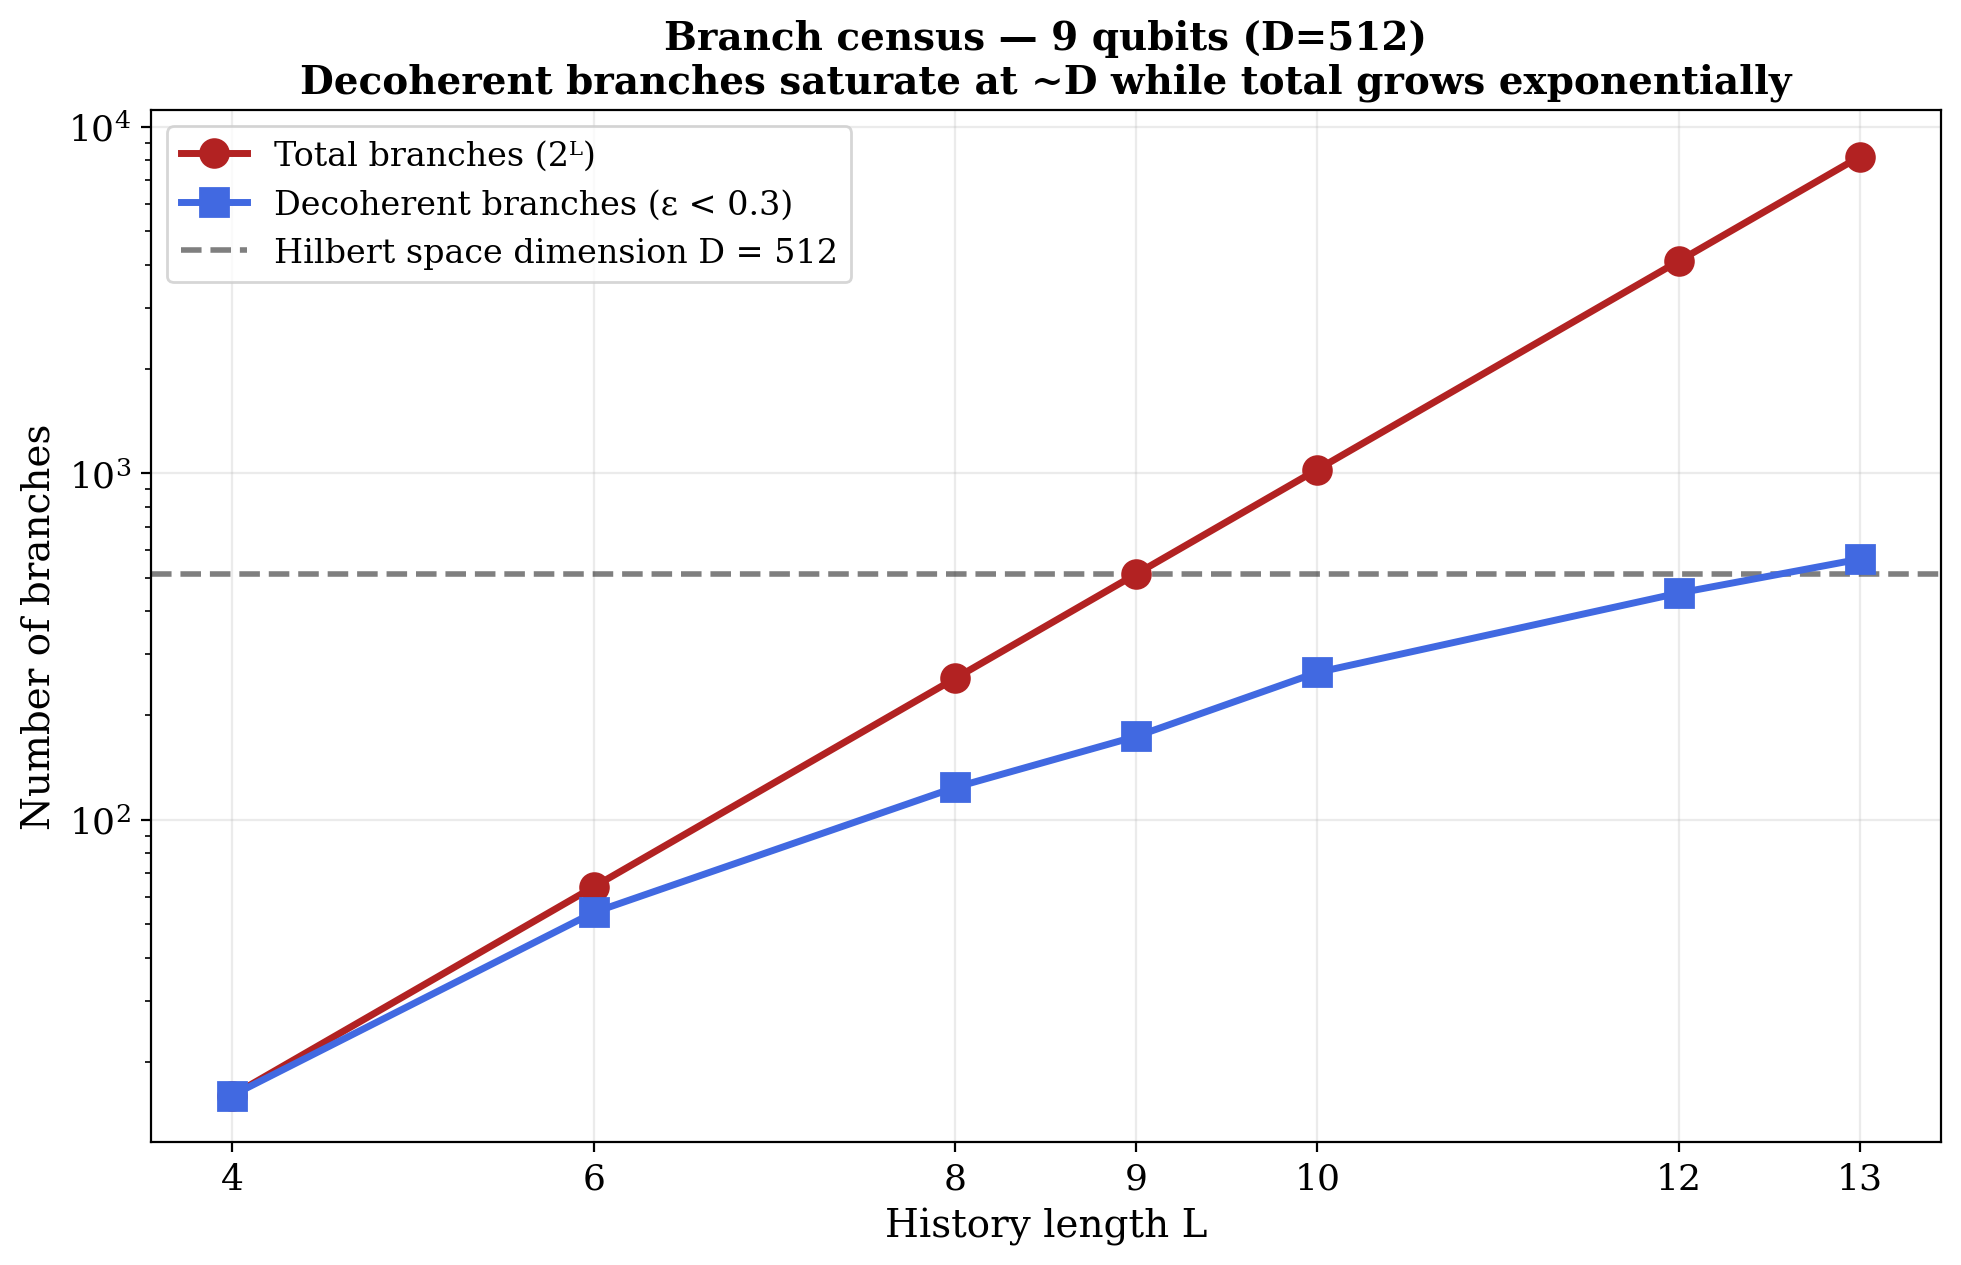
\includegraphics[width=0.7\textwidth]{../results/branch_census.png}
  \caption{Branch census: total branches (red) versus decoherent branches with
    $\varepsilon < 0.3$ (blue). Growth slows dramatically around
    $D = 512$ (black dashed), while total branches grow as $2^L$.}
  \label{fig:census}
\end{figure}

Figure~\ref{fig:survivors} shows the frequency distribution of the survivors.
The distribution of decoherent branches matches a binomial with Born probability
$p_1 = 0.746$, not the combinatorial distribution $\binom{L}{n_1}/2^L$ that would
arise from naive branch counting. The process is not literally i.i.d.; the binomial
arises as the Born-rule prediction for the frequency distribution of surviving
branches.

\begin{figure}[H]
  \centering
  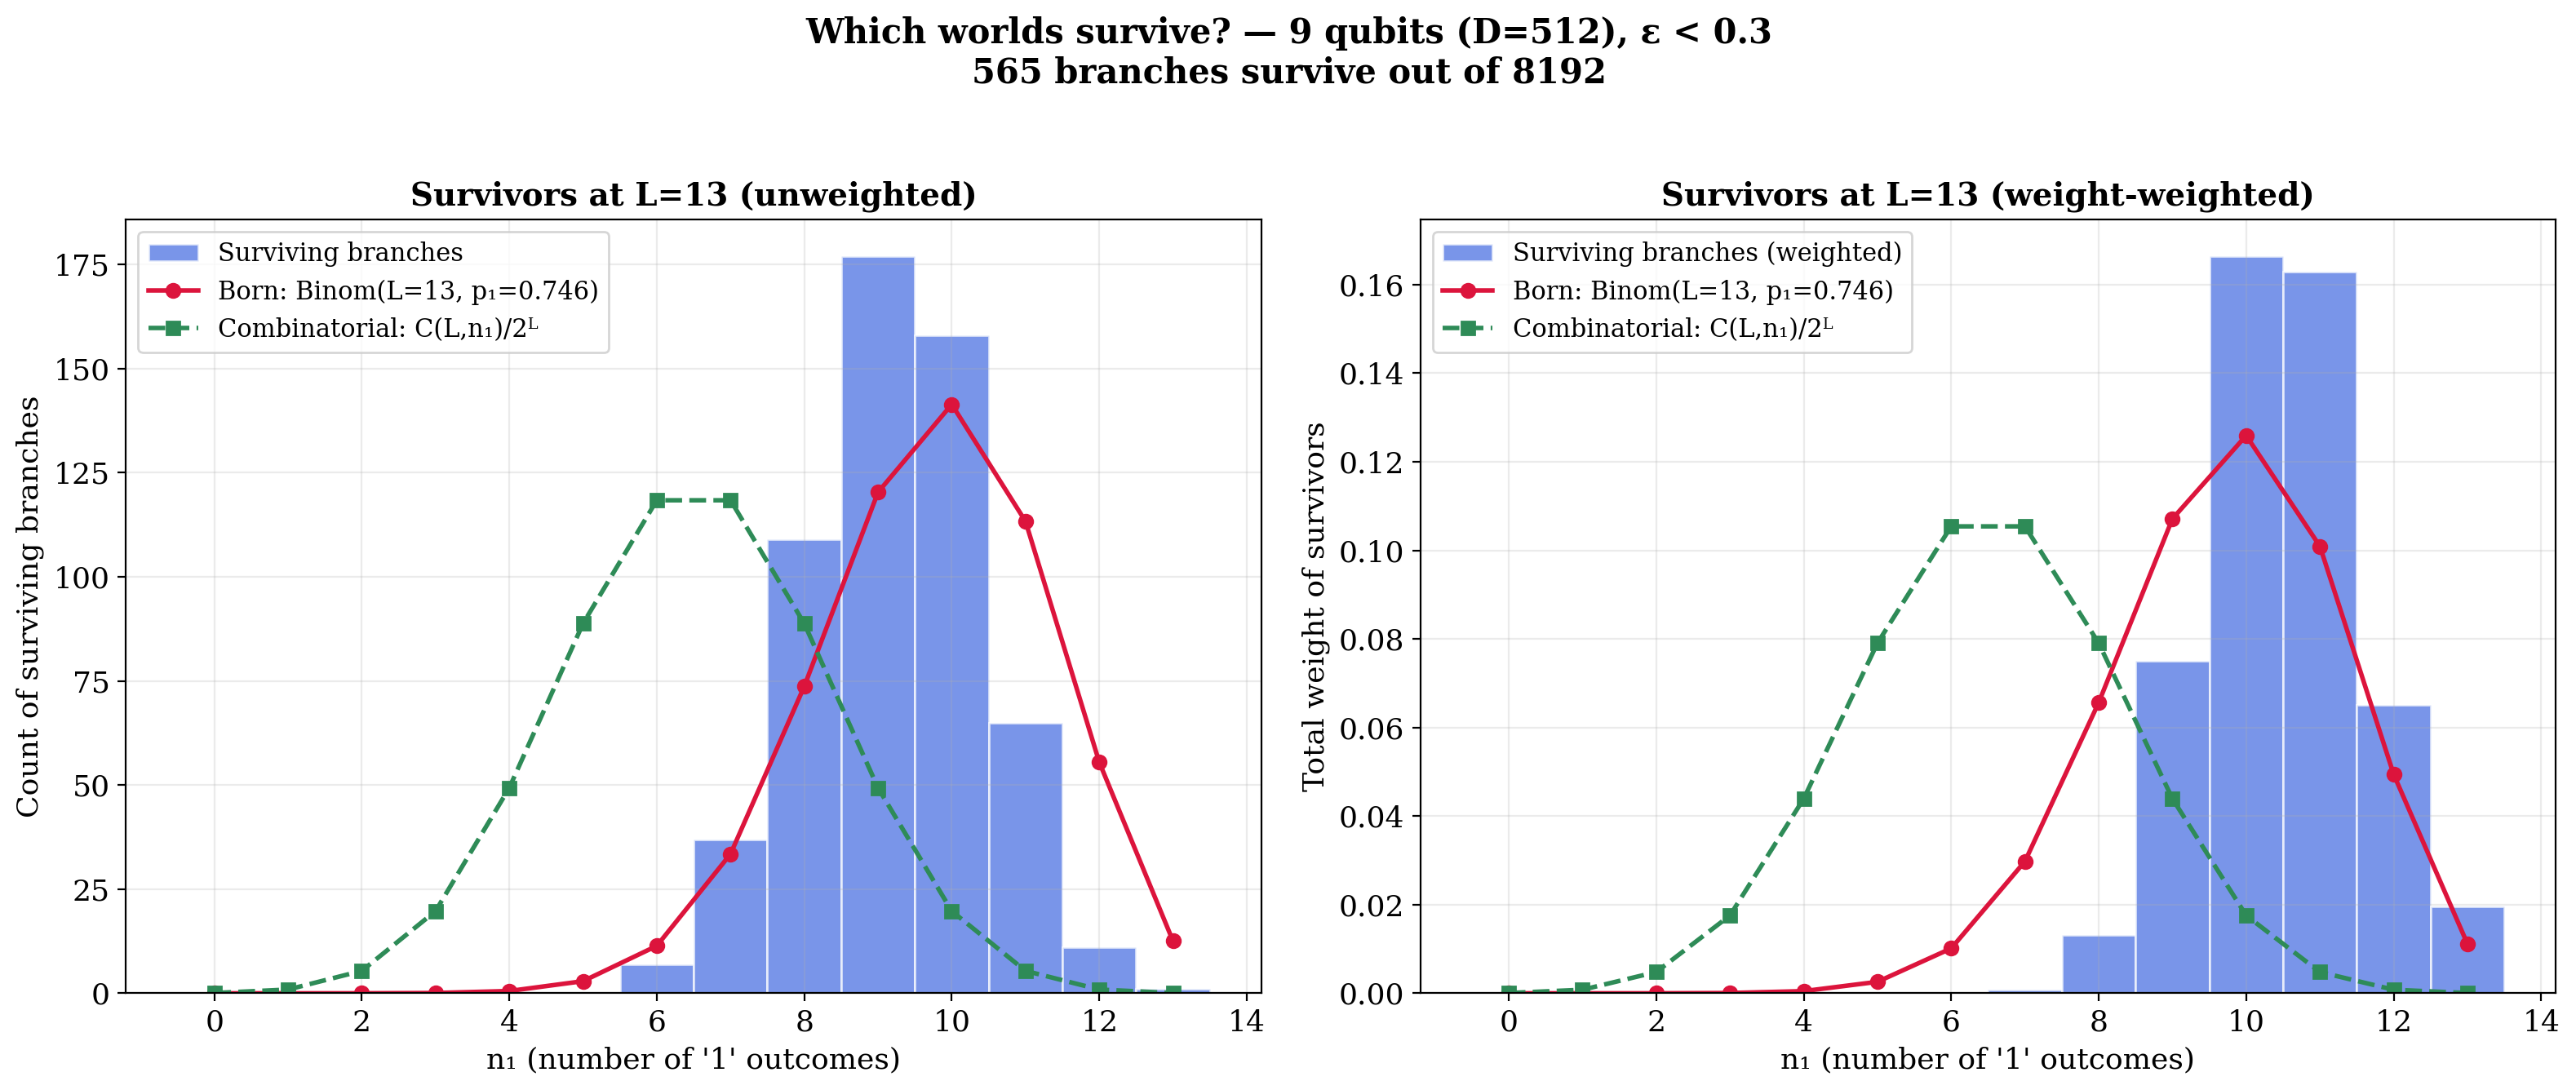
\includegraphics[width=0.95\textwidth]{../results/branch_survivors.png}
  \caption{Frequency histogram of surviving branches at $L = 12$. Left: unweighted
    count. Right: weighted by branch norm. The red curve shows the Born binomial
    $\text{Binom}(L, p_1)$; the green curve shows the combinatorial distribution.
    Survivors follow Born, not branch counting.}
  \label{fig:survivors}
\end{figure}

\subsection{The All-Zeros and All-Ones Asymmetry}
\label{sec:asymmetry}

Two extreme branches tell the story most vividly.

The \emph{all-tails} branch---tails on every single flip. This is the most
anti-Born history possible. Its weight is $2 \times 10^{-8}$ (essentially zero),
and its $\varepsilon = 0.77$---it overlaps heavily with neighboring branches and
fails the approximate decoherence criterion by a wide margin.

The \emph{all-heads} branch---heads every time. There is only one such history
out of 4096, so by branch counting it is just as rare as all-tails. But the coin is
loaded 75\% heads, so this outcome is not absurd. Its weight is 0.025
(a million times larger than all-tails), and its $\varepsilon = 0.20$---it
remains approximately decoherent. It has no siblings with the same frequency to
compete with, so it retains its share of the Hilbert space.

In this model, anti-Born branches do not just have low weight. They also fail the
approximate decoherence criterion used to identify distinct record-bearing
histories.

\subsection{The Gram Matrix}
\label{sec:gram}

Figure~\ref{fig:gram} shows the overlap between every pair of branches at
$L = 10$ (1024 branches), arranged by frequency. Dark means low overlap; bright
means high overlap. The Born-frequency blocks are dark---those branches remain
approximately orthogonal. The combinatorial-peak blocks are bright---those
branches overlap significantly.

\begin{figure}[H]
  \centering
  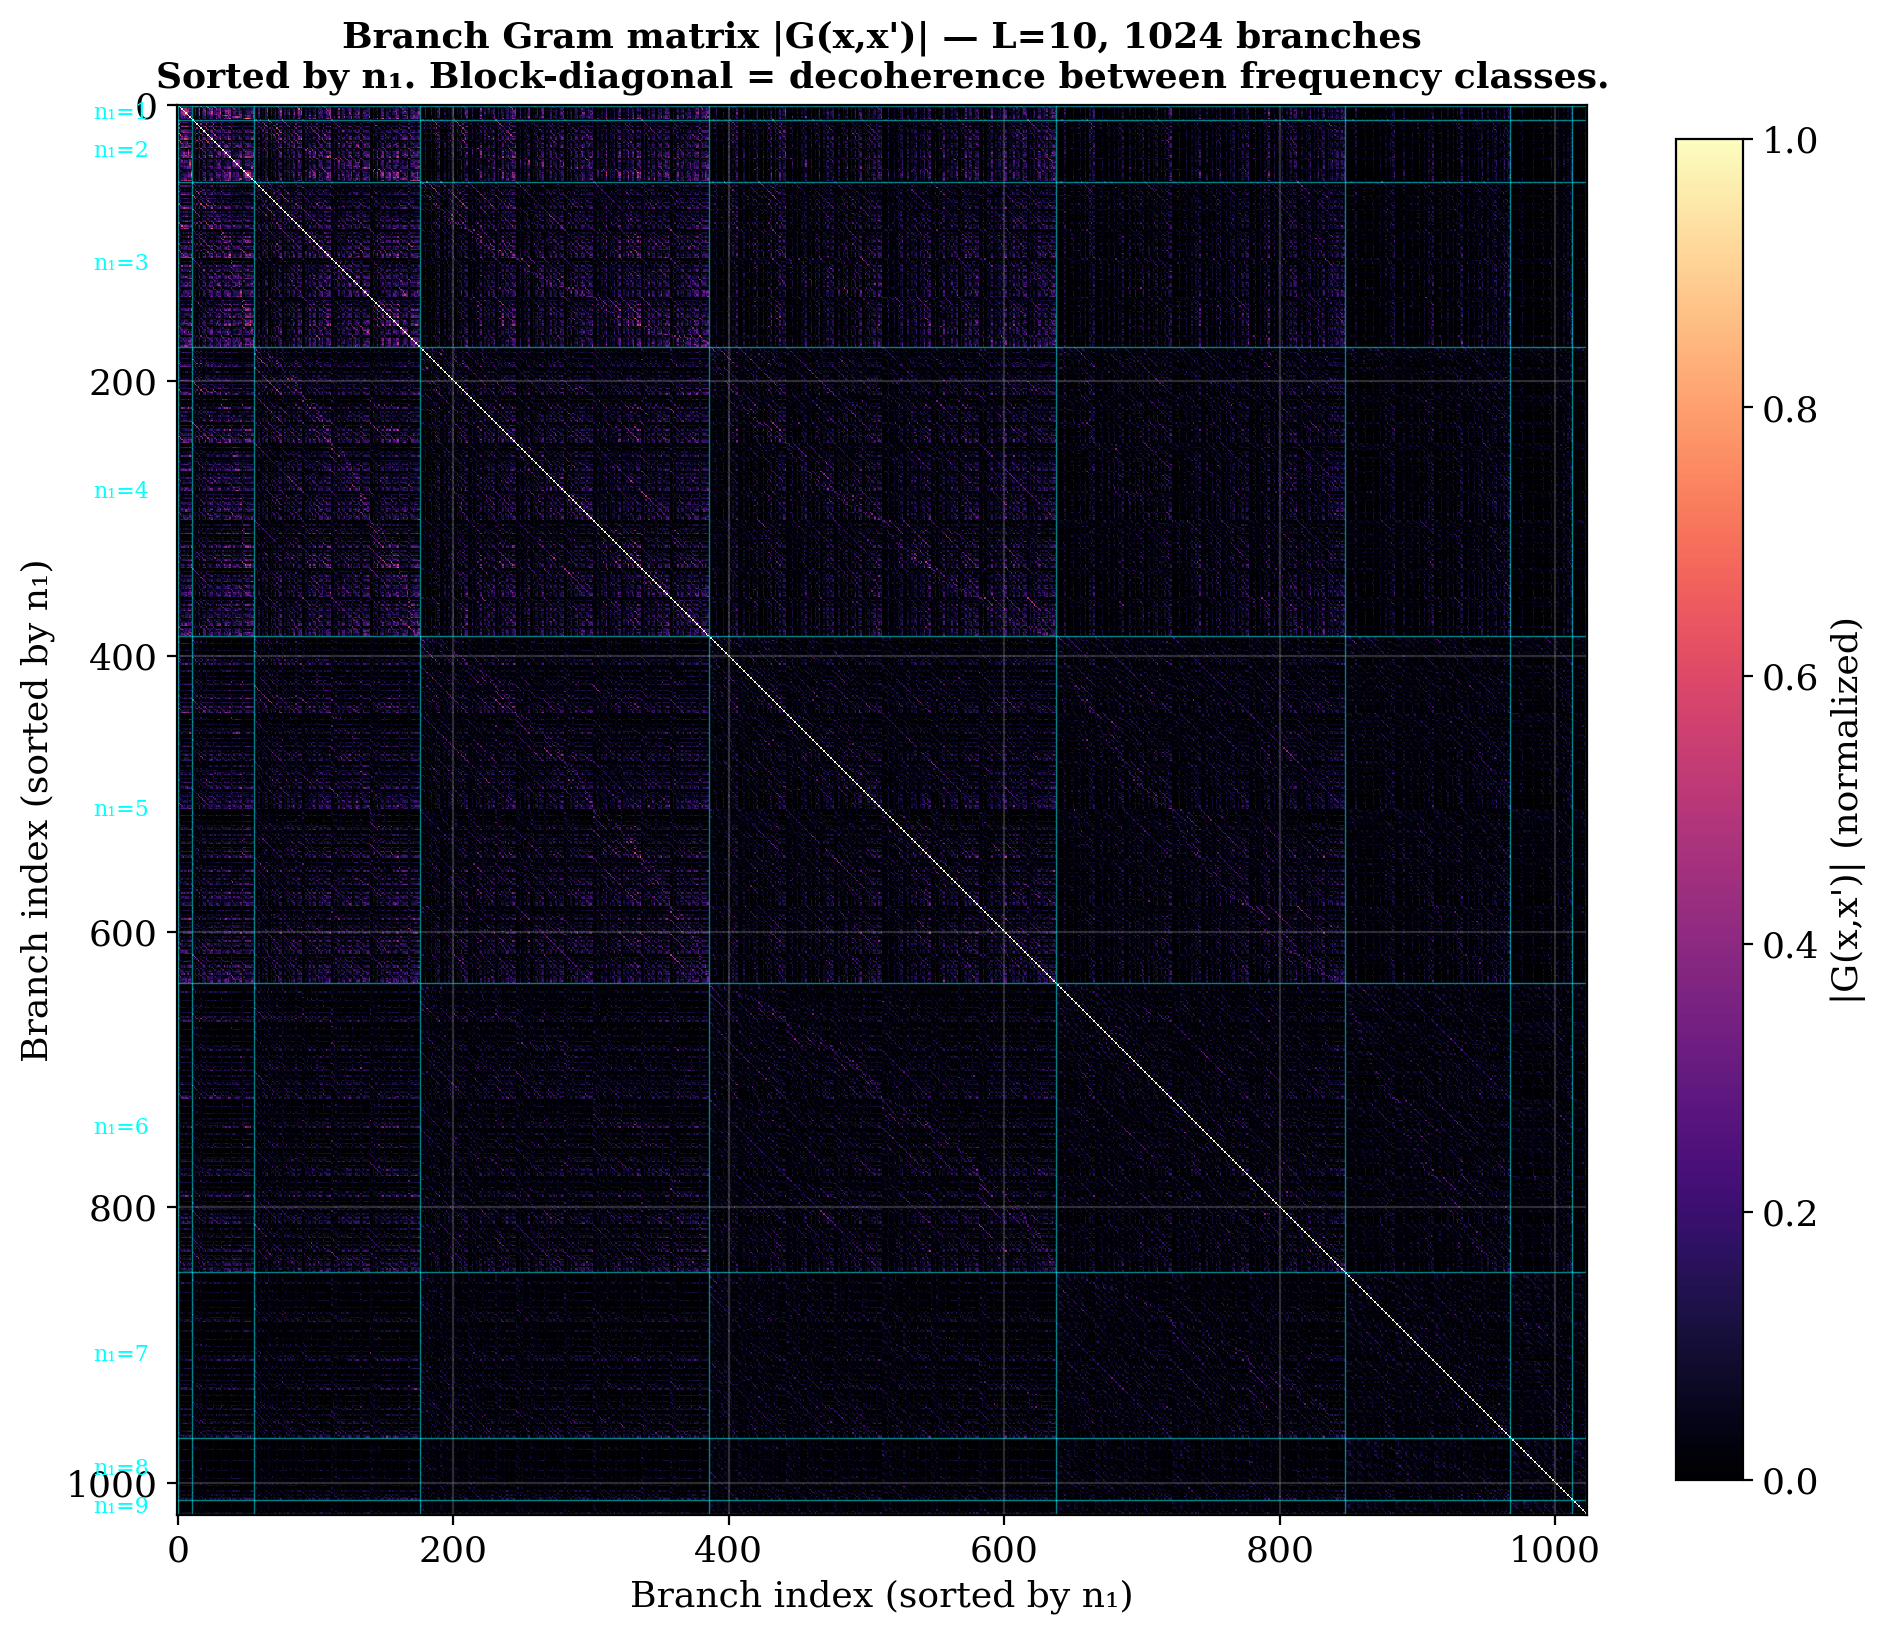
\includegraphics[width=0.7\textwidth]{../results/branch_gram.png}
  \caption{Absolute value of the normalized Gram matrix for 1024 branches at
    $L = 10$, sorted by $n_1$. Block-diagonal structure reflects frequency-class
    grouping. Brighter off-diagonal elements indicate recoherence. The central
    (combinatorial-peak) blocks are more coherent than the Born-frequency blocks.}
  \label{fig:gram}
\end{figure}

\subsection{Individual Branches}
\label{sec:one-reality}

Finally, we pick four individual branches and trace their evolution step by step
(Figure~\ref{fig:one-reality}).

Each row shows one branch's outcome sequence, how its running frequency $n_1(k)/k$
evolves flip by flip, and its weight $\|\psi(\mathbf{x},k)\|^2$ at each step.
The Born-typical branch sees its frequency converge to 75\% and retains significant
weight. The anti-Born branches drift toward 50\% and their weight drops by many
orders of magnitude.

\begin{figure}[H]
  \centering
  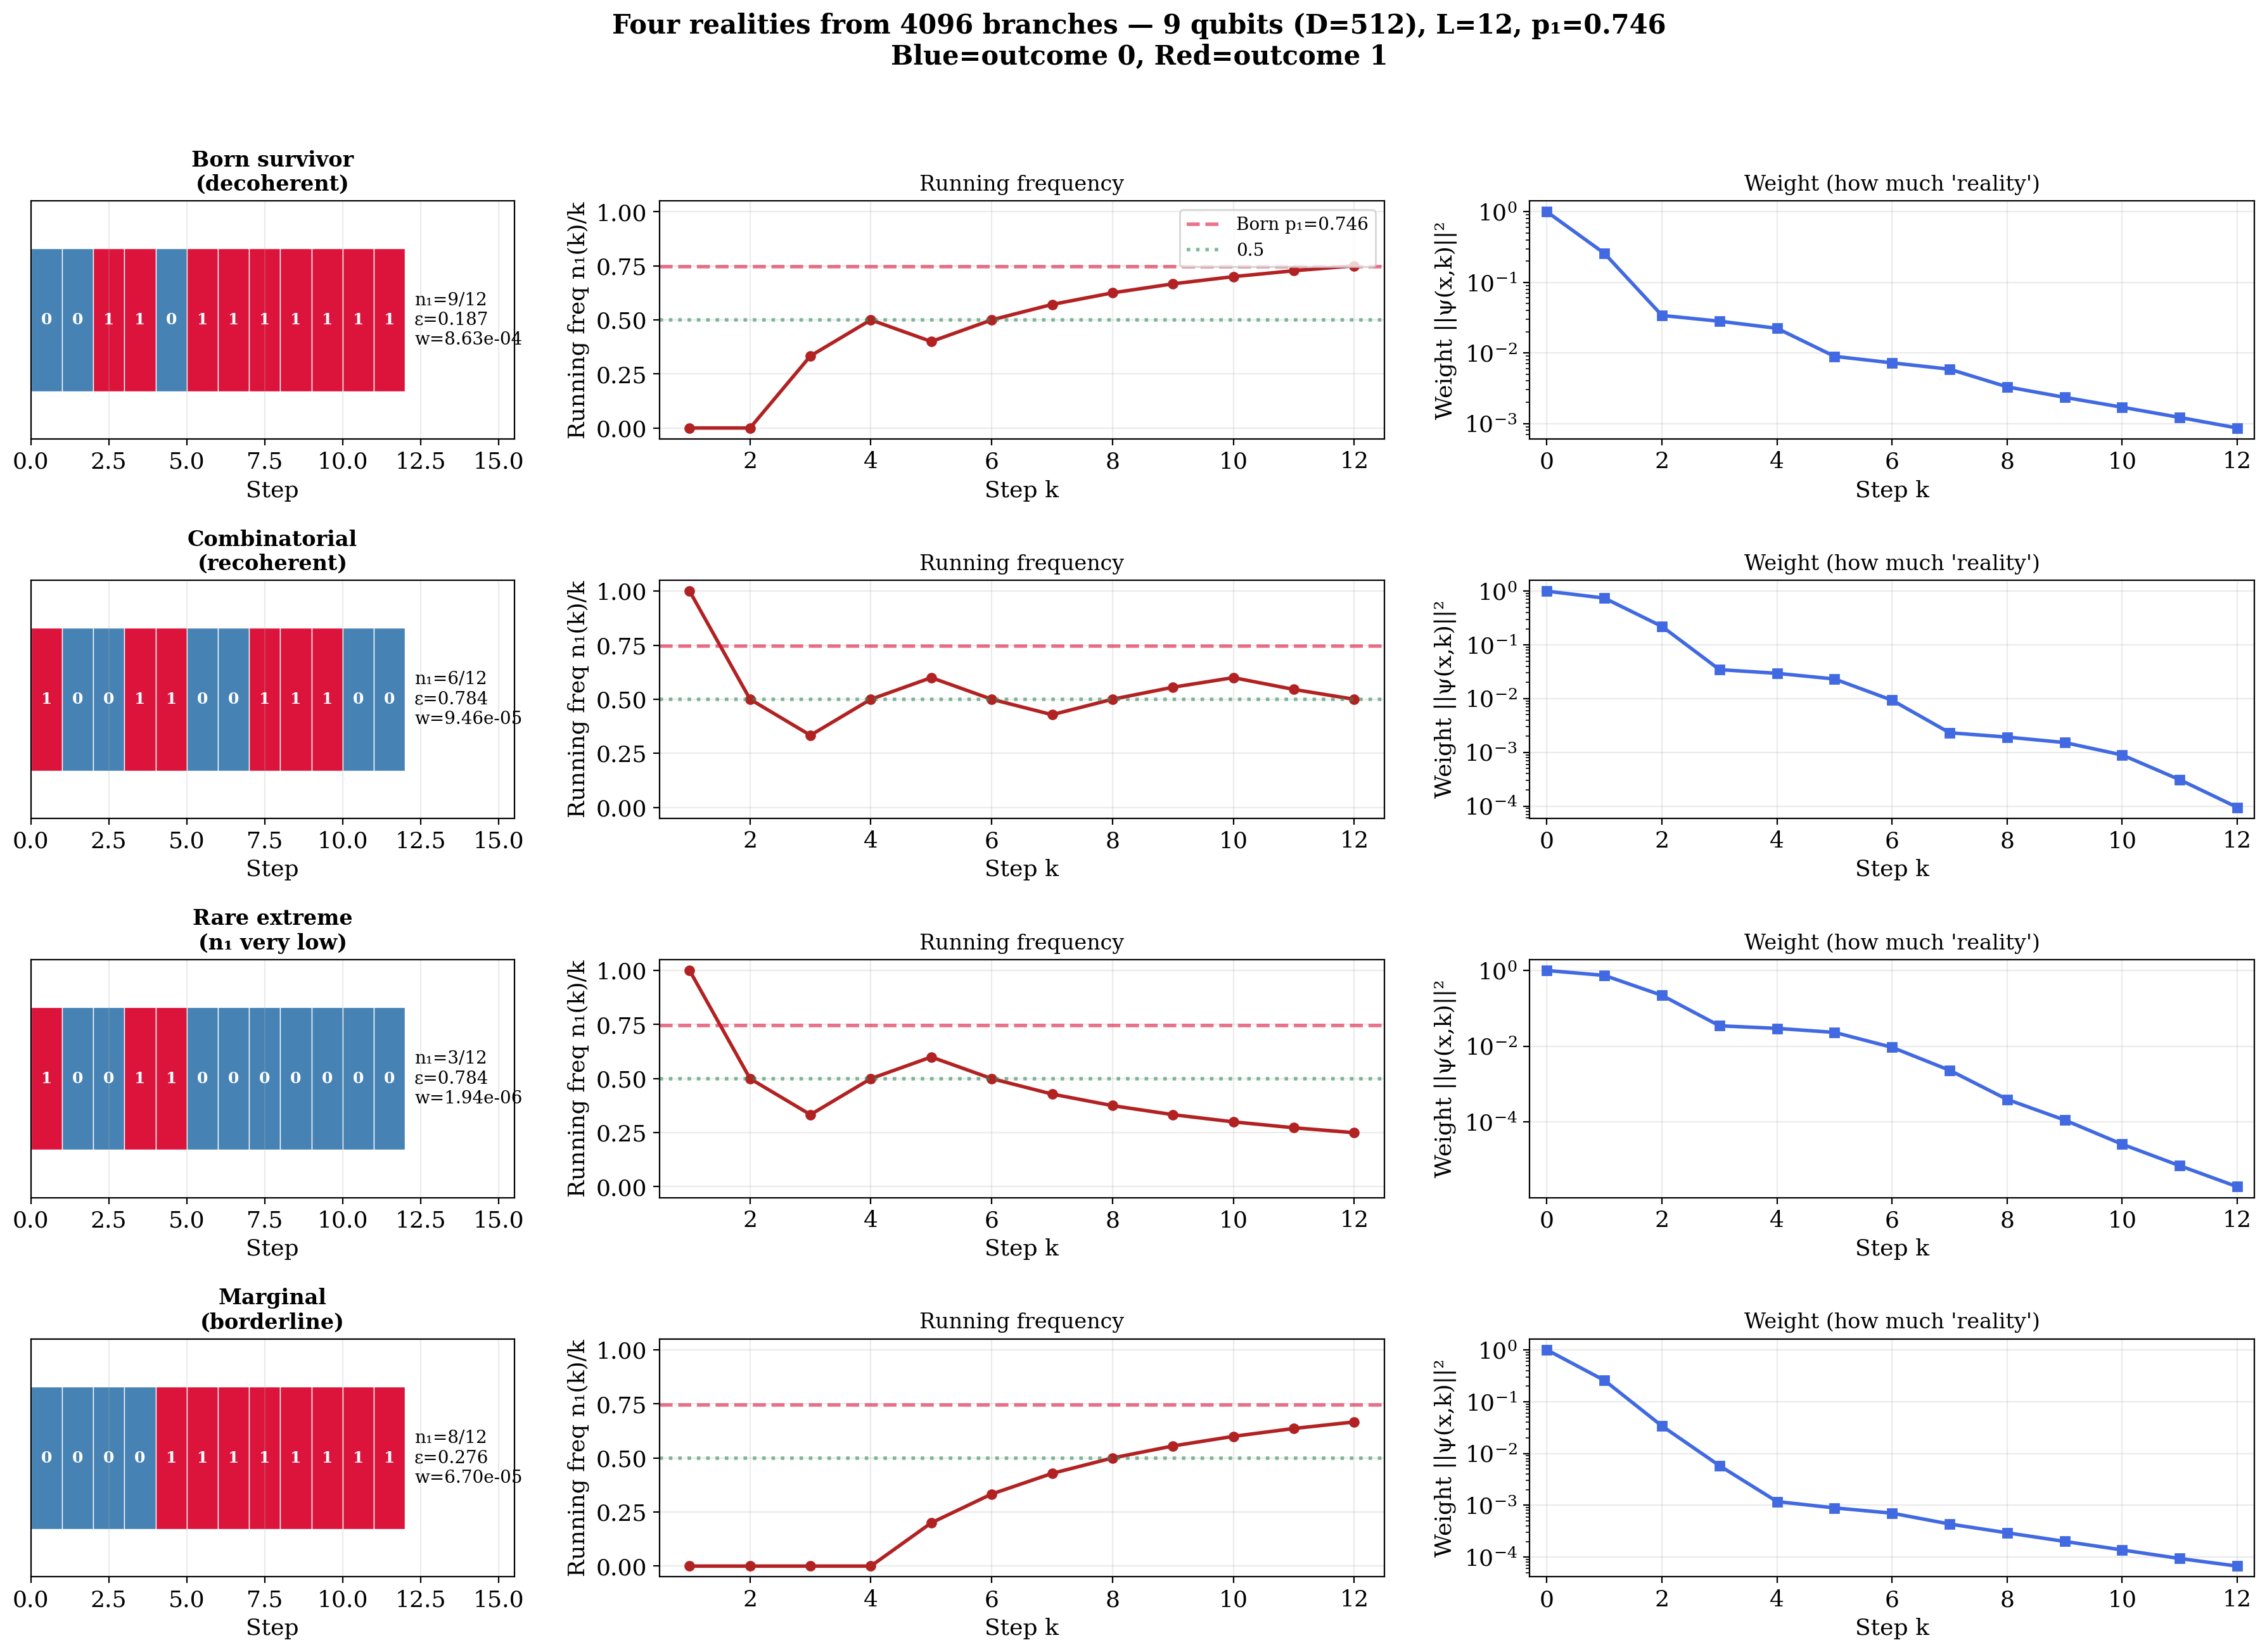
\includegraphics[width=0.95\textwidth]{../results/one_reality.png}
  \caption{Four representative branches at $L = 12$. Each row shows: the
    outcome sequence (blue = 0, red = 1), the running frequency $n_1(k)/k$
    converging (or not) to $p_1$, and the branch weight $\|\psi(\mathbf{x},k)\|^2$
    at each step.}
  \label{fig:one-reality}
\end{figure}


% ============================================================================
\section{Limitations}
\label{sec:limitations}
% ============================================================================

This work has clear limitations.

\begin{itemize}
  \item \textbf{Small system.} Nine qubits ($D = 512$) is tiny. Real physical
    systems have Hilbert spaces of exponentially large dimension. We cannot say
    whether the $3.1\times$ gap grows, shrinks, or stays constant as $D$ increases.
    Strasberg's analytical results~\citep{Strasberg2024} suggest it should improve,
    scaling as $D^{-\alpha}$, but we have not verified this numerically.

  \item \textbf{Classical simulation only.} We simulate the full state vector on a
    classical computer. This limits us to small systems. A quantum computer could
    in principle probe larger Hilbert spaces, but the analysis requires tracking
    exponentially many branches, which is inherently hard.

  \item \textbf{Not a proof.} We demonstrate the effect for one Hamiltonian
    (transverse-field Ising) with one coarse-graining (Hamming weight).
    We have not proven that Born-rule filtering occurs for all Hamiltonians
    or all reasonable coarse-grainings.

  \item \textbf{Specific coarse-graining.} The Hamming-weight threshold $\geq 4$
    gives $p_1 = 0.746$. Different thresholds give different $p_1$, and we have not
    systematically explored the dependence on the coarse-graining.

  \item \textbf{Time-step dependence.} The Born--combinatorial gap depends on
    $\Delta t$, requiring sufficient evolution between projections for the
    dynamics to spread correlations. The reported $3.1\times$ gap is specific to
    $\Delta t = 1.2$.

  \item \textbf{Integrable dynamics.} Our transverse-field Ising Hamiltonian is
    integrable (solvable by Jordan-Wigner transformation), unlike the chaotic
    random matrix models used by Strasberg. The filtering pattern appears
    nonetheless, suggesting the mechanism may not require chaos---but this also
    means we cannot claim to have tested it in a chaotic regime.

  \item \textbf{No environment.} Real decoherence involves tracing out an
    environment. Our system has no environment---the 9 qubits are the whole
    universe. This is intentional (it matches Strasberg's formalism, where the
    system itself is the recorder), but it is a simplification.
\end{itemize}


% ============================================================================
\section{Conclusion}
\label{sec:conclusion}
% ============================================================================

In a 9-qubit transverse-field Ising chain with exact unitary evolution, the
recoherence parameter $\varepsilon$ dips near the Born frequency with a
$3.1\times$ gap over the combinatorial peak, matching the qualitative shape
reported by Strasberg and collaborators in random matrix models. At the
individual-branch level, the finite Hilbert space preferentially preserves
Born-typical branches while anti-Born branches lose approximate decoherence. This
is consistent with Strasberg's analytical results and extends the qualitative
picture from random matrices to a local, physically motivated Hamiltonian.

A natural next step is to test the filtering mechanism in a lattice gauge theory,
where the factored Hilbert space and local gauge constraints are physically
motivated, and where the coarse-graining is dictated by the gauge
symmetry---charge sectors, flux sectors---rather than chosen by hand. If the
pattern survives when the projectors are fixed by gauge invariance rather than
selected by the experimenter, the case for a physically grounded mechanism
becomes considerably stronger.



% ============================================================================
% References
% ============================================================================

\bibliographystyle{unsrtnat}

\begin{thebibliography}{10}

\bibitem[Everett(1957)]{Everett1957}
H.~Everett.
\newblock ``Relative State'' Formulation of Quantum Mechanics.
\newblock \emph{Reviews of Modern Physics}, 29(3):454--462, 1957.

\bibitem[Wallace(2012)]{Wallace2012}
D.~Wallace.
\newblock \emph{The Emergent Multiverse: Quantum Theory According to the Everett
  Interpretation}.
\newblock Oxford University Press, 2012.

\bibitem[Carroll(2019)]{Carroll2019}
S.~Carroll.
\newblock \emph{Something Deeply Hidden: Quantum Worlds and the Emergence of
  Spacetime}.
\newblock Dutton, 2019.

\bibitem[Deutsch(1999)]{Deutsch1999}
D.~Deutsch.
\newblock Quantum Theory of Probability and Decisions.
\newblock \emph{Proceedings of the Royal Society A}, 455(1988):3129--3137, 1999.

\bibitem[Zurek(2005)]{Zurek2005}
W.~H.~Zurek.
\newblock Probabilities from Entanglement, Born's Rule $p_k = |\psi_k|^2$ from
  Envariance.
\newblock \emph{Physical Review A}, 71:052105, 2005.

\bibitem[Griffiths(1984)]{Griffiths1984}
R.~B.~Griffiths.
\newblock Consistent Histories and the Interpretation of Quantum Mechanics.
\newblock \emph{Journal of Statistical Physics}, 36(1--2):219--272, 1984.

\bibitem[Gell-Mann and Hartle(1990)]{GellMannHartle1990}
M.~Gell-Mann and J.~B.~Hartle.
\newblock Quantum Mechanics in the Light of Quantum Cosmology.
\newblock In W.~H.~Zurek, editor, \emph{Complexity, Entropy, and the Physics of
  Information}, pages 425--458. Addison-Wesley, 1990.

\bibitem[Strasberg and Schindler(2023)]{StrasbergSchindler2024}
P.~Strasberg and J.~Schindler.
\newblock Shearing off the tree: Emerging branch structure and Born's rule in
  an equilibrated multiverse.
\newblock arXiv:2310.06755, 2023.
\newblock (Replaced and extended by arXiv:2601.19703.)

\bibitem[Strasberg et~al.(2024)]{Strasberg2024}
P.~Strasberg, T.~E. Reinhard, and J.~Schindler.
\newblock First principles numerical demonstration of emergent decoherent
  histories.
\newblock \emph{Physical Review X}, 14:041027, 2024.
\newblock DOI: 10.1103/PhysRevX.14.041027.

\bibitem[Strasberg et~al.(2026)]{Strasberg2025}
P.~Strasberg, J.~Schindler, J.~Wang, and A.~Winter.
\newblock Approximate decoherence, recoherence and records in isolated quantum
  systems.
\newblock arXiv:2601.19703, 2026.

\end{thebibliography}


% ============================================================================
\appendix
\section{Interpretive Notes}
\label{sec:interp}
% ============================================================================

\emph{These are personal, speculative notes---not part of the core result. They
record how the author reads the filtering mechanism and where it might connect to
open questions in quantum foundations. They go beyond what Strasberg and
collaborators claim.}

\bigskip

\subsection{Collapse as Identity, Not Process}

In the standard story, wave function collapse is something that \emph{happens}:
at the moment of measurement, the superposition is somehow reduced to a single
outcome. The Everett picture removes this event but replaces it with a question:
why does each branch-observer see Born-rule statistics?

Our toy model suggests a possible reframing. In the simulation, the coarse-graining
(the ``observer'') is a fixed projection---a particular way of carving up the
Hilbert space into ``outcomes.'' The system evolves unitarily. The projections
define what counts as a branch. And the finite geometry of the Hilbert space
constrains which branches can coexist as approximately decoherent histories.

If this picture generalizes, collapse would not be a process that happens at a
moment in time, but a statement about which patterns of outcomes can be sustained
as separate, non-interfering histories in a finite-dimensional space. In our
9-qubit model, the Born-typical patterns survive and the anti-Born patterns do
not.

\subsection{The Hamiltonian Constrains the Basis}
\label{sec:basis}

A natural objection: who chose the projection? Why Hamming weight and not some other
decomposition of the Hilbert space?

In our experiment, the choice was guided by two criteria from Strasberg's framework:
the projector should be \emph{coarse} (high rank, so that each subspace is large
enough for the dynamics to spread correlations within it) and \emph{compatible with
the symmetry structure} of the Hamiltonian. The Hamming-weight threshold $\geq 4$
satisfies both: it partitions $D = 512$ into subspaces of dimension 382 and 130,
and total magnetization is a natural collective observable for an Ising chain.

Not every decomposition works. We verified that tracking a single qubit (two rank-256 projectors,
$d_0 = d_1 = 256$) produces $\varepsilon \approx 1$ everywhere---no
filtering, no stable branches. The reason is intuitive: a single qubit scrambles
completely between steps, so successive projections carry no
memory. The Hamming-weight projector averages over all 9 qubits, which smooths out
the fast single-qubit fluctuations and preserves enough structure for the filtering
to appear.

We did not systematically search over all possible coarse-grainings, so we cannot
claim that Hamming weight is uniquely selected. But the contrast between
``coarse projector shows filtering'' and ``fine projector does not'' is consistent
with Strasberg's framework, in which the Hamiltonian constrains which
decompositions support approximately decoherent histories.

\subsection{Anti-Born Branches: Not Just Unlikely, But Indistinct}

The usual explanation for why we do not see anti-Born statistics is that those
branches have low squared amplitude---they are ``unlikely.'' The filtering
mechanism suggests something additional. In our simulation, the anti-Born branches
do not just have low weight---they also lose approximate decoherence, overlapping
significantly with neighboring branches.

The all-zeros branch is a concrete example. Its weight is
$2 \times 10^{-8}$, and its recoherence parameter is 0.77: it shares most of
its overlap structure with neighboring branches. Whether this loss of decoherence
constitutes a loss of ``separate reality'' depends on interpretive commitments
we do not adjudicate here. But numerically, these branches fail the standard
decoherent-histories criterion for classicality.

This observation---that anti-Born branches lose decoherence, not just
weight---shifts the emphasis from ``how likely is this branch?'' to ``does this
branch maintain the approximate decoherence needed for stable records?''

\subsection{Local Couplings}

One might worry that the filtering pattern depends on the non-local, all-to-all
coupling of random matrix Hamiltonians. Our Ising example provides one data point
against this: the ZZ couplings are nearest-neighbor only, and the single-qubit
fields are local. This is a baby lattice model with the same tensor-product
structure $\mathcal{H} = \bigotimes_i \mathcal{H}_i$ that underlies lattice field
theory. The fact that the qualitative filtering pattern appears with local gates
is suggestive, though a single 9-qubit example obviously cannot establish
generality.

\subsection{Finite Dimensions as Physics, Not Limitation}

Strasberg's mechanism requires finite $D$. This might seem restrictive, since
textbook quantum field theory uses infinite-dimensional Fock spaces. But any lattice
regularization of a quantum field theory lives in a finite-dimensional factored
Hilbert space $\mathcal{H} = \bigotimes_x \mathcal{H}_x$, and physical
arguments---the Bekenstein bound, holographic entropy bounds---independently suggest
that the Hilbert space accessible to a bounded region is finite-dimensional. The
mechanism does not require $D$ to be small, only finite. A lattice gauge theory
would provide the natural next test: finite $D$, local tensor-product structure,
and a coarse-graining dictated by gauge invariance rather than chosen by hand.

\subsection{Relation to Bohmian Mechanics}

Bohm's pilot-wave theory (1952) shares the single-thread intuition: one
definite configuration is real at all times, and Born's rule emerges dynamically
rather than by postulate. Two features were always seen as weaknesses: particle
position is the preferred variable \emph{by fiat}, and the guiding equation is an
extra dynamical law beyond Schr\"odinger.

The recoherence picture, if it generalizes, removes both. The Hamiltonian selects
the coarse-graining basis (Section~\ref{sec:basis}): the preferred observable is
derived, not chosen. And no guiding equation is needed---unitary evolution is the
complete dynamics. In Bohm's framework, Born's rule requires assuming the initial
particle distribution is $|\psi|^2$-distributed; in the recoherence framework,
filtering is geometric---branches that violate Born statistics lose approximate
decoherence regardless of the initial state.

Whether one thread is actual (as Bohm proposed) or all Born-typical threads are
equally real (as Everett proposed) is not decided by the mechanism. But what Bohm
had to postulate---a preferred variable and a statistical equilibrium---the finite
geometry constrains.

\subsection{The Remaining Question}

Even if the filtering mechanism generalizes, it would not explain why \emph{you}
are in \emph{this} particular branch. The mechanism, if it holds, would explain
why the surviving branches have Born-typical statistics. It would not explain why
you experience one branch rather than another. That question may be about indexical
identity rather than physics, but we note it as an open issue rather than
dismissing it.

But the picture, if it holds, is suggestive: the wave function evolves
unitarily---as Everett proposed---yet only Born-typical branches remain
approximately decoherent, and an observer would simply be one such branch.
Collapse, in this reading, is not something that happens but the fact that you are
one projection, experiencing one sequence of outcomes. If that framing survives
scrutiny, then Copenhagen and Everett may both have been pointing at the same
structure from different angles.

\end{document}
